% arara: latexmk : {options: ["-xelatex", "-synctex=1", "-shell-escape"]}

% options:
% thesis=B bachelor's thesis
% thesis=M master's thesis
% czech thesis in Czech language
% english thesis in English language
% hidelinks remove colour boxes around hyperlinks

\documentclass[thesis=M,czech]{template/FITthesis}[2019/12/23]

\usepackage[utf8]{inputenc}

\usepackage{dirtree}

\newcommand{\tg}{\mathop{\mathrm{tg}}} %cesky tangens
\newcommand{\cotg}{\mathop{\mathrm{cotg}}} %cesky cotangens

% % % % % % % % % % % % % % % % % % % % % % % % % % % % % % 
% ODTUD DAL VSE ZMENTE
% % % % % % % % % % % % % % % % % % % % % % % % % % % % % % 

\department{Katedra softwarového inženýrství}
\title{Návrh a implementace aplikace pro dobrovolnickou brigádu SummerJob}
\authorGN{Matyáš} %author's given name/names
\authorFN{Ješina} %author's surname
\authorWithDegrees{Bc. Matyáš Ješina} %author's name with academic degrees
\author{Matyáš Ješina} %author's name without academic degrees
\supervisor{Ing. Marek Jílek}
\acknowledgements{Děkuji všem a za vše. Nevíte-li, co sem napsat, příkaz odstraňte.}
\abstractCS{Práce se zabývá návrhem a implementací frontendové i backendové části systému pro dobrovolnickou brigádu SummerJob. Výsledkem práce je webová aplikace, která umožňuje správu brigádníků, oblastí, jednotlivých prací, dopravních prostředků potřebných pro výkon prací a dalších souvisejících částí. Nejprve je provedena analýza stávajícího řešení, jeho problémů a nedostatků, následně jsou prozkoumány možnosti pro vývoj nové aplikace. Na základě analýzy požadavků a technologií je poté implementována nová webová aplikace. Dále se práce zabývá také vytvořením automatického plánovacího systému, který umožňuje přiřazovat brigádníky na jednotlivé práce podle zadaných parametrů. Poslední část je věnována testování a nasazení aplikace na produkční server.}
\abstractEN{Doplňte ekvivalent abstraktu Vaší práce v~angličtině.}
\placeForDeclarationOfAuthenticity{V~Praze}
\declarationOfAuthenticityOption{2} %volba Prohlášení
\keywordsCS{webová aplikace, SummerJob, Next.js, Javascript, brigáda.}
\keywordsEN{Final Thesis, \LaTeX{}.}
\website{https://github.com/jesinmat/summerjob/} %volitelná URL práce, objeví se v tiráži


\begin{document}

\begin{introduction}
	Zde doplňte úvod Vaší práce.
\end{introduction}
\chapter{Cíl práce}

Cílem práce je návrh a implementace webové aplikace pro dobrovolnickou brigádu SummerJob. 

Daný systém musí evidovat registrované účastníky, oblasti, ve kterých se daný rok pracuje, jednotlivé práce, které se v rámci oblastí vykonávají a
dopravní prostředky, které je možné použít k přepravě brigádníků na místo. Na základě těchto informací poté organizátoři akce vybírají práce na
jednotlivé dny, přiřazují k nim brigádníky a plánují dopravu. Pro podporu plánovacího procesu bude vytvořen automatický plánovací systém,
který na základě dostupných prací v daném dni přiřadí brigádníky k práci na základě jejich preferencí a dostupnosti. Tento plánovací systém musí být snadno
rozšiřitelný či zcela nahraditelný, aby bylo možné jej snadno optimalizovat bez nutnosti úpravy zbytku systému.

Systém musí být dostupný primárně pro organizátory akce a umožňovat vygenerování plánu v tisknutelném formátu. Webová aplikace musí být dostupná
i na mobilních zařízeních, pokud by bylo nutné provést změny v plánu na místě.

Aby bylo možné systém dále rozšiřovat, například přidáním mobilní aplikace, musí být k dispozici podrobně zdokumentované API umožňující kompletní
přístup k funkcím systému.
\chapter{Současné řešení}

Pro evidenci dat a plánování pracovních činností se v současné době používá interní aplikace JobsPlanner, která využívá technologii .NET. Tato aplikace je dostupná pouze pro počítače se systémem
Windows. Zdrojový kód nebyl v době psaní práce k dispozici. Dále je možné využít jednoduché webové rozhraní pro zápis účastníků, prací a aut. Webová část také umožňuje tisk hotových plánů.

\section{Nevýhody současného řešení}

Na základě analýzy aplikace a konzultací s organizátory akce SummerJob byly zjištěny následující nedostatky současného řešení:

\begin{itemize}
    \item Aplikace je dostupná pouze na počítačích se systémem Windows.
    \item Aplikace neumožňuje práci více uživatelů současně.
    \item Aplikace využívá jednotný účet pro přístup k databázi pro všechny uživatele, není tedy možné rozdělit práva jednotlivým organizátorům.
    \item Spojení s databází je zajištěno přes otevřený port databáze dostupný z internetu. Toto řešení je z hlediska bezpečnosti nevhodné.
    \item Spojení s databází často vypadává. V takovém případě není možné s aplikací pracovat.
    \item Automatické plánování trvá příliš dlouho, v některých případech i minutu.
    \item Není k dispozici API pro přístup k datům.
    \item Pro každý ročník je nutné založit novou databázi a ručně překopírovat potřebná data.
    \item Webové rozhraní nabízí pouze omezenou funkcionalitu.
    \item Zdrojový kód webového rozhraní využívá proprietární nezdokumentovaný framework, což znemožňuje jeho rozšíření.
    \item Brigádníci nemají možnost zobrazit si svůj plán či upravit své osobní informace.
\end{itemize}

Vzhledem k rostoucí popularitě akce SummerJob a s tím souvisejícím rostoucím počtem účastníků se dané problémy projevují stále výrazněji.
Je tedy nutné vytvořit nové řešení, které tyto nedostatky odstraní.

\chapter{Analýza a návrh}

Tato kapitola popisuje proces analýzy požadavků a návrhu systému.
V první části jsou popsány metody použité při analýze požadavků. V druhé části jsou popsány návrhy systému, které byly vytvořeny na základě analýzy požadavků.
Analýza je nezávislá na technologiích použitých při následné implementaci.

\section{Analýza požadavků}

Analýza požadavků je proces, který má za cíl získat informace o požadavcích na systém. Na základě průběžných konzultací s vedoucím práce, Ing. Markem Jílkem, a 
Bc. Lucií Annou Procházkovou, členy týmu organizátorů akce SummerJob, byly získány podrobné informace o procesu organizace akcí a požadované funkcionalitě nové aplikace.
Tyto konzultace byly prováděny i dále během vývoje systému, aby bylo zajištěno, že systém bude plnit požadavky organizátorů akce. Pomocí této agilní metody
bylo možné průběžně reagovat na případné změny a seznamovat budoucí uživatele s aktuálním stavem systému.

V této práci bude kromě obecných pojmů pro jednotlivé součásti systému použita také existující terminologie z akce SummerJob: \textit{pracant} je označení pro brigádníka, \textit{job} je označení pro práci, kterou brigádník vykonává.

\subsection{Funkční požadavky}
\label{sec:functional-requirements}

Funkční požadavky popisují funkcionalitu požadované aplikace, specifikují možnosti, vlastnosti a operace, které musí být možné provádět.
Jsou základem při návrhu a implementaci systému.

\begin{itemize}
    \item \textbf{FP1. Přihlášení a registrace:} uživatelé systému musí být schopni se přihlásit do systému, pokud jsou registrováni v právě probíhajícím ročníku. Registraci není třeba implementovat, probíhá externě a schvalují ji organizátoři akce.
    \item \textbf{FP2. Správa oprávnění a uživatelských účtů:} uživatelé systému mají různá oprávnění, která určují, co všechno mohou v systému provádět. Oprávnění jsou rozdělena podle přístupu ke správně jednotlivých položek (pracanti, joby, auta, plánování). Administrátor má možnost nastavit oprávnění jednotlivým uživatelům, případně uživateli zcela zakázat přístup do systému.
    \item \textbf{FP3. Správa pracantů:} organizátoři akce musí být schopni spravovat seznam pracantů. Musí být možné přidávat, mazat a upravovat informace o pracantech. Tyto informace zahrnují jméno a příjmení, e-mail, telefonní číslo, alergie, dostupnost pracanta v jednotlivých dnech akce, informaci, zda a kdy se chce pracant účastnit adorací. Organizátoři sami během akce pracují a patří tedy mezi pracanty.
    \item \textbf{FP4. Správa jobů:} organizátoři akce musí být schopni spravovat seznam jobů. Musí být možné přidávat, mazat a upravovat informace o jobech. Tyto informace zahrnují název jobu, popis jobu, lokalitu, kontaktní osobu, alergeny na místě, celkový počet pracantů, které je možné přiřadit k jobu, požadovaný počet silných pracantů a počet dní nutných na splnění práce. U prací je evidována dostupnost občerstvení a sprchy. Jednotlivé joby musí být možné označit jako splněné, případně prioritní. Prioritní joby musí být v seznamu jobů odlišeny od ostatních a slouží ke zvýšení viditelnosti prací, které jsou pro organizátory důležité. V jobech musí být možné vyhledávat.
    \item \textbf{FP5. Správa aut:} organizátoři mohou spravovat dostupná auta. U aut se eviduje počet míst, vlastník (pracant) a najeté kilometry. Na základě najetých kilometrů během akce se po skončení akce počítá kompenzace pro řidiče. Systém by měl umožnit evidenci, zda byla kompenzace vyplacena.
    \item \textbf{FP6. Správa plánů:} zodpovědné osoby mohou tvořit plány na jednotlivé dny, přidávat joby do plánů, přidávat pracanty do jobů, plánovat dopravu pro jednotlivé joby. Pracanti z různých jobů mohou sdílet dopravu. Systém musí podporovat současnou práci více uživatelů během tvorby plánu. Plány musí být možné zobrazit v tisknutelném formátu.
    \item \textbf{FP7. Automatický plánovač:} systém musí být schopný na žádost oprávněného uživatele naplánovat rozvrh pracantů na zadané joby. Po přidání jobů do plánu a vyžádání vygenerování plánu plánovač přiřadí pracanty na joby a naplánuje dopravu. Přitom respektuje dostupnost pracantů v daný den, alergie, požadovaný počet silných pracantů na jobu a požadavky na adoraci.
    \item \textbf{FP8. Správa ročníků:} systém musí být schopný spravovat více ročníků akce SummerJob. Administrátor systému má možnost přepínat mezi jednotlivými ročníky. Každý ročník má název a časové rozpětí.
    \item \textbf{FP9. Správa oblastí:} systém musí být schopný spravovat oblasti, do kterých jsou joby rozděleny. U oblasti se eviduje nutnost dopravy autem a možnost adorace. Oblasti jsou vztaženy k aktuálnímu ročníku.
    \item \textbf{FP10. Záznam systémových změn:} systém musí být schopný zaznamenávat změny, které uživatelé provádějí. Záznamy musí obsahovat časové razítko, uživatele, který změnu provedl a popis změny. Administrátor má možnost zobrazit záznamy změn.
    \item \textbf{FP11. API:} systém poskytuje API, které umožňuje přístup k datům systému. API musí umožňovat provádět operace na úrovni srovnatelné s webovou aplikací.
\end{itemize}

\subsection{Nefunkční požadavky}

Nefunkční požadavky se týkají výkonu, spolehlivosti, bezpečnosti, škálovatelnosti a dalších aspektů systému. Nepopisují funkce systému, ale zaměřují se na celkovou kvalitu, provozuschopnost a výkonnost.

\begin{itemize}
    \item \textbf{NP1. Bezpečnost:} systém bude využívat přihlášení a ověření práv uživatelů pro přístup k datům. Uživatel bez potřebného oprávnění nesmí mít přístup datům, pro které je dané oprávnění nezbytné. Výjimkou je přístup k datům potřebným pro vykonávání činností, na které má uživatel oprávnění, například přístup ke jménům pracantů při přidávání nového auta do systému za účelem určení majitele. Přístup k databázi nebude možný přímo z internetu, ale pouze přes webovou aplikaci nebo API. Spojení mezi uživatelem a aplikací musí být šifrované.
    \item \textbf{NP2. Udržovatelnost a rozšiřitelnost:} výsledná aplikace využívá rozšířené technologie a standardy, které umožňují další rozšíření. K dispozici je dokumentace popisující fungování aplikace a použité technologie. Vývojáři systému mají možnost snadno rozšiřovat aplikaci o nové funkce.
    \item \textbf{NP3. Nezávislost na platformě:} aplikace nesmí být vázána na konkrétní operační systém. Vývojáři systému mají možnost snadno přenést aplikaci na jinou platformu. Webová aplikace musí být responzivní a použitelná na současných mobilních zařízeních i počítačích.
    \item \textbf{NP4. Rychlost plánovače:} plánovač musí být schopen vygenerovat plán pro 150 pracantů a 50 jobů do 15 sekund.
\end{itemize}

\section{Návrh systému}

V této kapitole je popsán návrh systému na základě provedené analýzy. Návrh popisuje celkovou architekturu systému, webovou aplikaci a API, databázi a plánovací systém.
Systém bude současně obsluhovat jednotky až desítky uživatelů, není tedy nutné řešit škálovatelnost. Vzhledem k povaze akce SummerJob, která zajišťuje práci
v malých vesnicích a obcích v jedné oblasti, není možné, že budou systém využívat stovky či tisíce uživatelů současně.

\subsection{Architektura systému}

Aby bylo možné k vytvořenému systému přistupovat z libovolného zařízení, bude uživatelské rozhraní implementováno jako responzivní webová aplikace. Serverová část 
bude poskytovat API pro přístup k datům uloženým v databázi. Automatický plánovač bude vyčleněn do samostatné služby, aby bylo možné v případě potřeby provádět
jeho aktualizaci bez nutnosti zásahu do webového serveru. Toto řešení umožní v případě nutnosti optimalizace vybrat libovolný jazyk a technologie pro implementaci plánovače.
Aby nedošlo k selhání komunikace mezi serverovou částí webové aplikace a plánovačem v případě dočasného výpadku plánovače nebo jeho nedostupnosti při plánování, bude komunikace
mezi těmito komponentami probíhat pomocí fronty zpráv. Komunikace mezi jednotlivými komponentami bude probíhat pomocí standardních protokolů a rozhraní, aby bylo možné
 části nahradit jinými, pokud vybrané komponenty nebudou vyhovovat.
Schéma architektury systému je na obrázku \ref{fig:architecture}.

\begin{figure}[h]
    \centering
    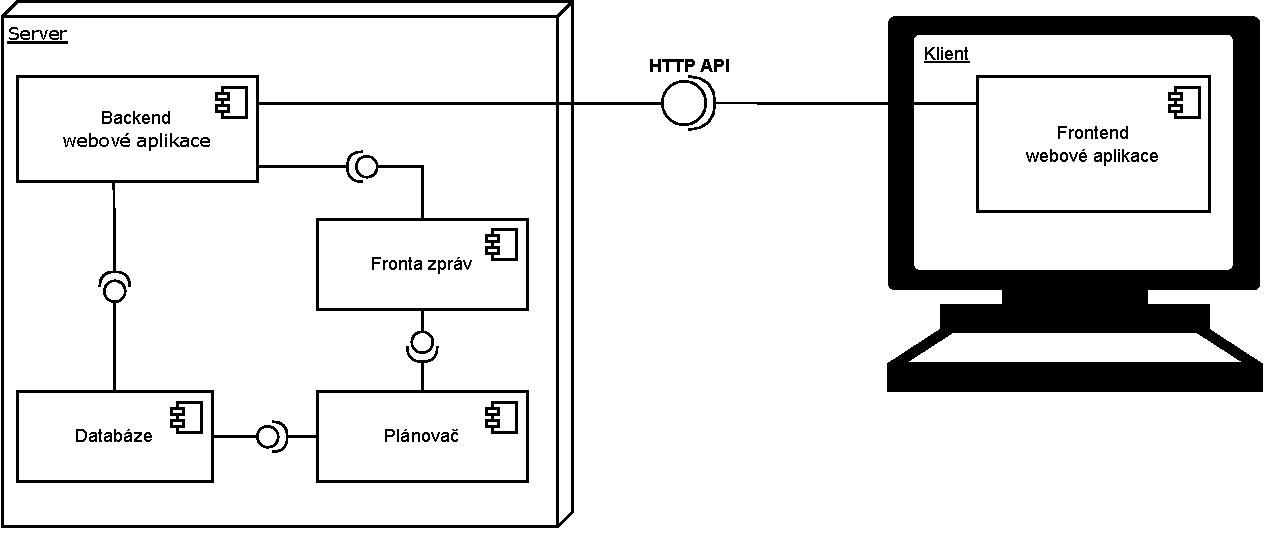
\includegraphics[width=\textwidth]{chapters/images/architektura}
    \caption{Architektura systému}
    \label{fig:architecture}
\end{figure}

\subsection{Webová aplikace a API}

Webová aplikace bude hlavním uživatelským rozhraním pro přístup k datům systému. Organizátoři budou přes webové rozhraní evidovat všechny potřebné údaje, vytvářet plány,
spravovat uživatelské účty, spouštět automatický plánovač a tisknout plány. K webové aplikaci budou účastníci i organizátoři přistupovat i přes mobilní zařízení během akce, 
je tedy nezbytné, aby byla aplikace responzivní. Serverová a klientská část webové aplikace budou splňovat všechny funkční požadavky, které jsou popsány v kapitole \ref{sec:functional-requirements}.
Funkční požadavek 11 dále určuje, že systém musí poskytovat API, které umožňuje přístup k datům systému. Aby bylo zajištěno,
že API poskytuje funkcionalitu shodnou s funkcionalitou webové aplikace, bude webová aplikace komunikovat se serverovou částí přes API.

Pro implementaci klientské části je vhodné využít moderní, udržované a dobře zdokumentované technologie. Akce SummerJob se často konají v pohraničních oblastech,
kde je možné, že uživatelé budou mít problémy s přístupem k internetu. Zvolené technologie musí umožňovat zotavení z chyb v případě nepodařených požadavků na server
a celkové množství přenesených dat by mělo být co nejmenší.

Přihlašování do webové aplikace je možné provést pomocí uživatelského jména a hesla, pomocí přihlašovacího odkazu nebo přes poskytovatele identity třetí strany.
Přihlašování pomocí uživatelského jména a hesla představuje největší bezpečnostní riziko, protože uživatelé mohou používat stejné heslo pro více služeb. Bylo by nutné
zajistit korektní správu hesel, jejich bezpečné ukládání a kontrolu. Dále by bylo nutné implementovat funkce pro obnovu hesla v případě zapomenutí.

Mezi poskytovatele identit patří například Google, Facebook nebo GitHub. Přihlašování přes poskytovatele třetí strany je výhodné pro uživatele, protože nemusí vytvářet
nový účet pro tuto aplikaci. Také nebude nutné v aplikaci zajišťovat správu a životní cyklus hesel. Tento způsob přihlašování však není vhodný pro uživatele,
kteří služby těchto poskytovatelů nevyužívají.

Přihlašování pomocí přihlašovacího odkazu zaslaného na e-mailovou adresu je vhodné pro uživatele, kteří nechtějí vytvářet nový účet a nechtějí používat služby poskytovatelů třetí strany.
V aplikaci nebude nutné implementovat funkce pro správu hesel, ale bude nutné implementovat funkce pro odesílání e-mailů. Všichni uživatelé musí při registraci na akci
vyplnit e-mailovou adresu, takže tato funkce bude dostupná pro všechny účastníky. Jedná se o preferované řešení. Pro implementaci této funkcionality může být využita
externí knihovna.

Aplikace slouží primárně pro organizátory akce. Volitelně je možné povolit přístup brigádníkům, kteří si v aplikaci mohou prohlížet přiřazenou práci na aktuální den a nastavit osobní údaje.
Pokud bude tato funkcionalita implementována, bude možné při dalším vývoji zpřístupnit pracovníkům další informace, např. nástěnku s informacemi.

\subsection{Databáze}

Databáze bude sloužit jako hlavní úložiště dat systému pro všechny potřebné údaje. Jedná se převážně o seznamy uživatelů, prací, aut, plánů a vazby mezi nimi.
Databáze bude uchovávat data o rozsahu několika stovek záznamů pro každý ročník. Běžné databázové systémy jsou schopny zpracovat takové množství dat, a tak není potřeba
klást na výběr databáze žádné specifické požadavky.

Na základě požadavků na aplikaci bylo vytvořeno konceptuální schéma, které je možné vidět na obrázku \ref{fig:schema}. Schéma zobrazuje vztahy mezi jednotlivými entitami a jejich atributy.
Schéma neobsahuje entity a atributy pro přihlašování do aplikace, protože tyto údaje budou v databázi uloženy pomocí zvolené knihovny.

\begin{figure}[h]
    \centering
    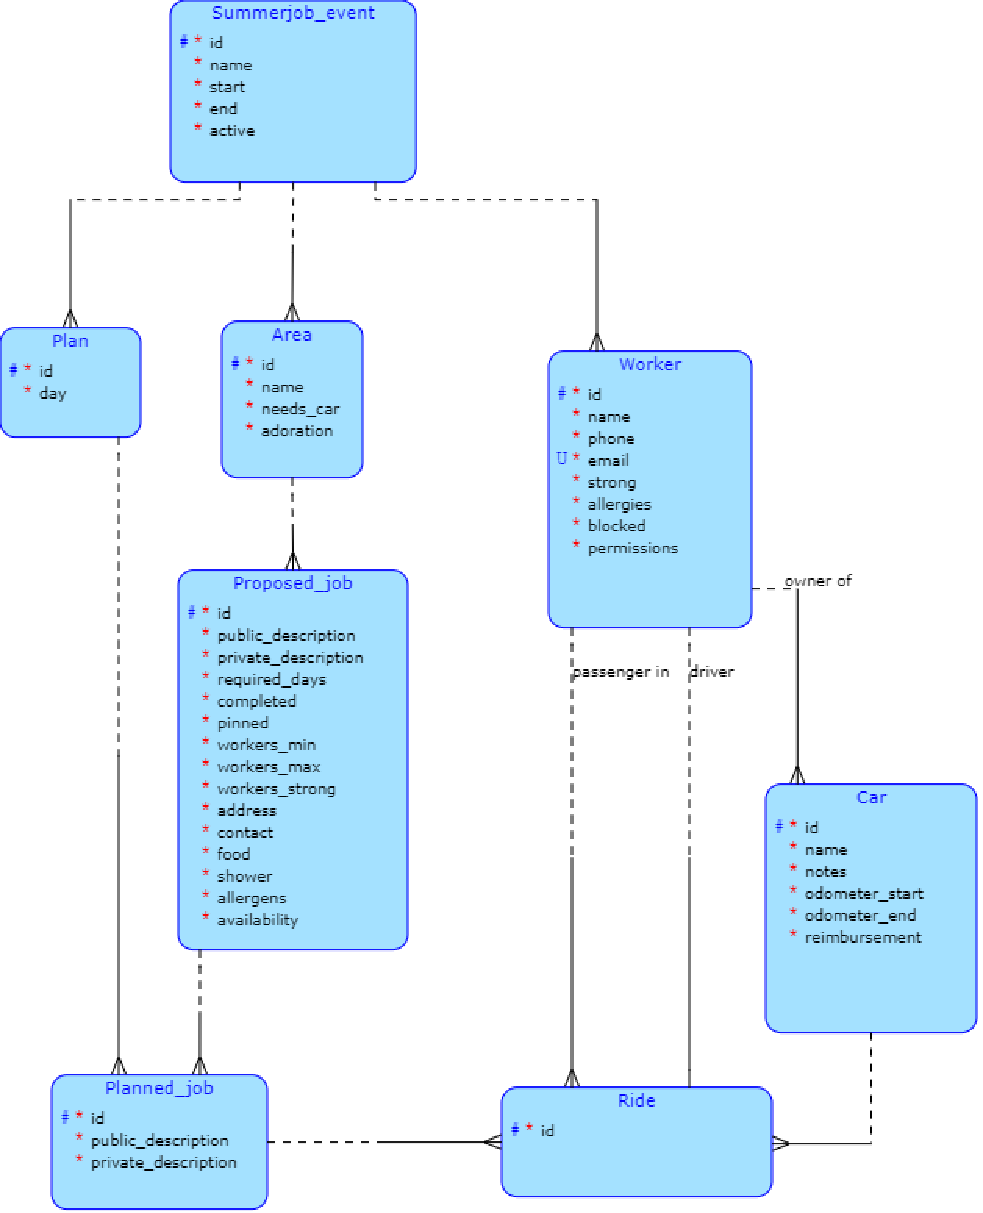
\includegraphics[width=\textwidth]{chapters/images/schema}
    \caption{Konceptuální schéma}
    \label{fig:schema}
\end{figure}


\subsection{Plánovací systém}

Automatický plánovací systém vychází z funkčního požadavku 7. Organizátoři budou mít možnost přidat do vytvořeného plánu na daný den požadované práce, které
chtějí vykonat. Tato funkce je implementována v rámci webové aplikace. Následně organizátor pomocí webové aplikace spustí proces plánování, který vygeneruje plán pro
daný den. Po dokončení se organizátorům zobrazí výsledný vygenerovaný plán.

Generování plánu zahrnuje přiřazení dostupných brigádníků k práci a přiřazení dopravy k práci, pokud je doprava vyžadována.
Plánovací systém tvoří plány podle následujících kritérií:
\begin{itemize}
    \item \textbf{Počet brigádníků na práci:} na zadanou práci musí být přiřazeno dostatečné množství brigádníků. Systém u každé práce eviduje minimální a maximální počet brigádníků, kteří mohou na místě pracovat. 
    \item \textbf{Počet silných pracantů:} na zadanou práci musí být přiřazeno dostatečné množství silných pracantů. Některé fyzicky náročné práce mohou vyžadovat přítomnost jednoho či více silných pracantů. Systém musí u každého brigádníka tento atribut evidovat.
    \item \textbf{Doprava:} pokud práce není v docházkové vzdálenosti od místa ubytování brigádníků, musí být brigádníkům přiřazena doprava. Systém musí u každé práce evidovat, zda je doprava vyžadována a u každého brigádníka evidovat, zda má k dispozici auto. Pokud je to možné, je pro práci vybrán brigádník s autem, který následně převáží ostatní brigádníky na pracoviště. Pokud jsou v autě volná místa, může řidič převážet i brigádníky z jiné práce, pokud je tato práce ve stejné oblasti jako práce řidiče (tzv. sdílená doprava).
    \item \textbf{Zodpovědný pracant:} na každou práci je zvolen jeden zodpovědný pracant, který zodpovídá za správné provedení práce a komunikuje s organizátory.
    \item \textbf{Alergie:} u práce je možné evidovat alergeny, které se na pracovišti nacházejí. Systém musí u každého brigádníka evidovat alergie a přiřazení brigádníka k práci musí být zajištěno tak, aby brigádník neměl alergii na alergeny na pracovišti.
    \item \textbf{Dostupnost pracantů:} někteří brigádníci mohou být v daný den nedostupní a nemohou se účastnit žádné práce. Systém musí u každého brigádníka evidovat, zda je v daný den dostupný. Pokud brigádník není v daný den dostupný, nesmí být přiřazen k žádné práci.
    \item \textbf{Adorace:} systém u brigádníků eviduje, zda se chtějí účastnit adorace. Adorace probíhá během dne v délce dvou hodin v některém z kostelů v okolí. Systém musí zajistit, aby brigádníci, kteří se chtějí účastnit adorace, byli přiřazeni k práci, která probíhá v blízkosti kostelu. Nejedná se o požadavek, který je nutné striktně dodržovat -- pracanta je možné přiřadit i k práci, která se nachází v jiné oblasti, pokud není možné přiřadit brigádníka k práci v blízkosti kostela. V takovém případě zobrazí webová aplikace upozornění.
    \item \textbf{Zachování naplánovaných prací:} pokud jsou před začátkem automatického plánování někteří brigádníci již přiřazeni k práci, musí být jejich přiřazení zachováno. Plánovací systém nesmí odebírat přiřazené brigádníky z práce, z naplánované dopravy atd. Může však přidávat nové brigádníky k práci nebo stávajícím pracantům přiřazovat dopravu, pokud není doprava již přiřazena.
\end{itemize}

Po vygenerování může být plán upraven organizátory pomocí webové aplikace. Do vygenerovaného plánu musí být možné přidat další práce a vyžádat nové plánování.
\chapter{Rešerše technologií}

V této kapitole je popsán výběr vhodných technologií pro implementaci systému. Dostupné technologie jsou uvažovány na základě předchozí analýzy.

\section{Webová aplikace a API}

Webová aplikace bude představovat hlavní rozhraní pro uživatele a společně s API představuje významnou část této práce.
Je proto nutné zaměřit se na výběr vhodné technologie, která umožní splnění všech zadaných požadavků.
Vzhledem k požadavkům na současnou práci více uživatelů při tvorbě plánu není možné využít generování statické webové stránky. Pro klientskou část
aplikace budou proto uvažovány technologie, které umožňují tvorbu dynamických webových aplikací.

Při výběru technologie hrála roli i oblíbenost a žádanost mezi vývojáři. Oblíbený nástroj s širokou komunitou často značí aktivní vývoj, kvalitní dokumentaci
a podporu. Dále je výhodou možnost využití statického typování, které zajišťuje větší bezpečnost a přehlednost kódu. Podle průzkumu Stack Overflow \cite{so_dev_survey} 
byl v minulém roce nejžádanějším frameworkem pro tvorbu webových aplikací React.js. Tento framework je postaven na jazyce JavaScript a umožňuje tvorbu klientských
dynamických webových aplikací. Nabízí také možnost využití statického typování pomocí nástroje TypeScript.

Mezi nejoblíbenějšími technologiemi s více než 1 000 hlasy se umístily také nástroje Svelte, ASP.NET Core a Next.js. Všechny zmíněné technologie umožňují tvorbu dynamických webových aplikací,
klientskou i serverovou část, nabízejí detailní dokumentaci a jsou aktivně vyvíjeny. Podporují také statické typování, částečné generování webových stránek na serveru (\textit{SSR} -- server side rendering),
serverový kód s podporou přístupu k databázi i tvorbu API.

Pro implementaci byl zvolen framework Next.js ve verzi 13. Tento framework využívá React.js pro tvorbu klientské webová aplikace a rozšiřuje jej o další funkce, například tvorbu API nebo pokročilejší nastavení serveru \cite{nextjs}.
V době psaní práce podporuje React 18 SSR pouze v beta verzi, Next.js proto nabízí ve výchozím nastavení původní generování webových stránek u klienta.
Během implementace však bude funkcionalita generování stránek na serveru využita, protože přináší výhody v rychlosti načítání stránky, možnosti kešování a spouštění kódu na serveru.

Pro přístup k databázi byl zvolen nástroj Prisma. Prisma umožňuje definovat schéma databáze v jednoduché textové podobě a pomocí automatického generování
příslušných typů pro TypeScript zajišťuje bezpečný přístup k databázi. Díky tomu je možné využít statické typování i při práci s databází, a to nejen 
pro navrácené typy, ale i pro tvorbu dotazů. Prisma také umožňuje tvorbu migračních skriptů, které zajišťují bezpečnou změnu schématu databáze. 

Pro zajištění správného zobrazení a funkcionality na mobilních zařízeních je nutné dodržovat principy responzivního designu. Pro zajištění kompatibility bude použit
framework Bootstrap, který nabízí responzivní kaskádové styly pro komponenty. Pro grafické elementy bude využit 
soubor ikon Font Awesome ve verzi 6.3, který nabízí širokou škálu ikon zdarma \cite{fontawesome}. Ikony jsou implementovány jako typ písma a klient tak nemusí stahovat jednotlivé obrázky.
Tato volba má za cíl minimalizovat objem přenesených dat a sjednotit vzhled ikon napříč aplikací.

\section{Plánovací systém}

Plánovací systém bude vytvořen v jazyce TypeScript s využitím nástroje Prisma. To umožní minimalizovat počet použitých technologií napříč projektem,
což zjednoduší jeho správu a údržbu. Při implementaci bude nutné vybrat vhodný algoritmus, aby bylo zajištěno splnění požadavku na rychlost.
Plánovač bude vytvořen jako samostatná komponenta, kterou bude možné v případě potřeby upravit přidáním vlastní implementace v jazyce TypeScript
či zcela nahradit jinou implementací. 
Pro přenos požadavků mezi webovým serverem a plánovacím systémem bude využita fronta zpráv.

\section{Fronta zpráv}

Fronta zpráv je datová struktura, která umožňuje asynchronní přenos zpráv mezi jednotlivými komponentami systému. Zprávy jsou ukládány do fronty
a následně zpracovány. V případě chyby je možné zprávu zpracovat znovu. Fronta zpráv je vhodným řešením pro přenos zpráv mezi webovým serverem a plánovacím systémem,
protože zajišťuje spolehlivý přenos zpráv v případě, že jedna ze služeb není v danou chvíli krátkodobě dostupná.

Službou pro poskytování fronty zpráv byla zvolena technologie RabbitMQ. Jedná se o open-source nástroj, který je dostupný zdarma. RabbitMQ je běžně používaným řešením
pro fronty zpráv \cite{rabbitmq} a využívá otevřený standard AMQP, jehož implementace je dostupná pro mnoho jazyků včetně TypeScriptu.

Frontu zpráv je možné nahradit jinou implementací, která bude splňovat požadavky na přenos zpráv. Fronta slouží pouze jako prostředník pro přenos zpráv mezi webovou aplikací
a plánovačem a nebude výrazně zatěžována, je tedy možné zvolit i jinou službu bez negativního dopadu na výkon systému.


\section{Databáze}

Pro výběr databáze byla na základě struktury dat zvolena technologie relačních databází. Uložená data mají pevně danou neměnnou strukturu,
jedná se o krátké textové řetězce, čísla a datum. Výhodou relačních databází je možnost snadno definovat vztahy mezi jednotlivými tabulkami,
což je v případě plánovacího systému nezbytné \cite{sql_nosql}. Dále je výhodou možnost využití transakcí, které zajišťují konzistenci dat.
Na základě analýzy a interních zkušeností administrátorského týmu akce SummerJob byl zvolen databázový systém PostgreSQL. Tento systém je
dostupný zdarma, má otevřený zdrojový kód a jedná se o běžně používané řešení s historií dlouhou více než 35 let \cite{postgresql}.
Podle uživatelského průzkumu Stack Overflow se v minulém roce jednalo o nejoblíbenější a nejžádanější databázový systém \cite{so_dev_survey_db}.

Objem dat a počet současných uživatelů systému je relativně malý, proto není nutné využívat technologie pro škálování databáze. Zálohování a obnova dat
je možná přes externí nástroje, které jsou také dostupné zdarma. Jedná se například o aplikaci pgAdmin, která umožňuje správu databáze přes grafické rozhraní.
Prisma podporuje PostgreSQL verze 9.4 a vyšší.

\section{Kontejnerizace}

Pro zajištění přenositelnosti a nezávislosti na platformě podle požadavku NF3 budou všechny komponenty systému spouštěny v kontejnerech \cite{what_is_container}.
Kontejnerizace je technologie, která umožňuje spouštět aplikace v izolovaném prostředí. Aplikace spuštěná v kontejneru je izolována od ostatních aplikací,
které jsou spuštěny na hostitelském operačním systému nebo v jiných kontejnerech. Kontejnery obsahují
všechny potřebné závislosti, které jsou nutné pro spuštění aplikace. Díky tomu je možné aplikaci spustit na libovolném operačním systému, který podporuje kontejnerizaci.

Pro kontejnerizaci byla zvolena technologie Docker. Jedná se o open-source nástroj, který je dostupný zdarma pro všechny běžné operační systémy.
V roce 2022 se jednalo o nejpoužívanější technologii pro kontejnerizaci \cite{docker_survey}.


\chapter{Implementace}

popsat vývoj webu, znova ukázat schéma db + ukázky Prismy, vysvětlit fungování Plánovače

Tato kapitola popisuje implementaci řešení. V první části je popsán vývoj klientské a serverové části webové aplikace včetně API, následující části se 
věnují implementaci Plánovače a kontejnerizaci.

\section{Vývoj webové aplikace}

Vývoj webové aplikace probíhal v iteracích, během kterých byly postupně implementovány jednotlivé funkce. Zástupci organizátorů akce SummerJob
měli k aplikaci přístup od začátku vývoje, což umožnilo průběžné testování a získávání zpětné vazby. Aplikace byla během vývoje dostupná na dočasné webové adrese.

Vybraný framework Next.js využívá rozšířenou verzi technologie React pro implementaci klientské části.
Pro zajištění správné funkcionality aplikace bylo nutné vytvořit několik vlastních komponent,
které jsou využívány v celé aplikaci. Jedná se zejména o tabulky se seznamy registrovaných brigádníků,
nabídek prací, evidencí aut a manuální úpravy plánu.
Klientská část webové aplikace je rozdělena do několika částí, které jsou popsány níže.

\subsection{Přihlašování}

Správa přihlašování je implementována pomocí knihovny NextAuth.js, která poskytuje rozhraní pro přihlašování pomocí různých poskytovatelů. Knihovna podporuje
přihlašování pomocí e-mailu, služeb Google, Facebook, GitHub, Twitter, Apple a dalších. Přihlašování pomocí uživatelského jména a hesla je autory knihovny 
považováno za nebezpečné a pro podporu je nutné implementovat vlastní ověření uživatelů. Na základě analýzy bylo proto zvoleno přihlašování pomocí e-mailu.

Přihlašování je první částí aplikace, která se zobrazí nepřihlášenému uživateli. Pokus o přístup na stránku, která vyžaduje přihlášení,
je zachycen na straně serveru a uživatel je přesměrován na přihlašovací stránku. Nedochází tedy k úniku citlivých dat nebo jiného interního obsahu.

Přihlašovací stránka obsahuje formulář s polem pro zadání e-mailové adresy. Po odeslání formuláře dojde k ověření existence uživatele v databázi.
Pokud je uživatel registrovaný v aktuálním ročníku akce a nejedná se o blokovaný účet, je uživateli odeslán e-mail s odkazem pro přihlášení a na stránce je 
zobrazena příslušná informace. Pokud uživatel neexistuje nebo je jeho účet blokovaný, je zobrazena chybová hláška.

Přihlášení pomocí odkazu v e-mailu je zabezpečeno pomocí jednorázového tokenu s omezenou časovou platností, který je generován při odeslání e-mailu.
Po přihlášení je token z databáze odstraněn.
Webovému prohlížeči je přiřazeno identifikační cookie s platností jeden měsíc, které je využíváno pro autentizaci uživatele. Během této doby se uživatel nemusí v
daném prohlížeči znovu přihlašovat. Platnost po dobu jednoho měsíce byla zvolena s ohledem na dobu trvání akce SummerJob -- jedná se o přípravu na ročník,
týden práce a čas pro vyřízení administrativy po skončení akce.

Cookie využívá atributy \texttt{HttpOnly} a \texttt{SameSite}, které zabraňují přístupu k hodnotě cookie ze skriptů a
pomáhají předcházet útokům typu CSRF. Dále je cookie chráněno proti úniku přes nezabezpečené připojení pomocí atributu \texttt{Secure}. 

Registrace dobrovolníků je řešena externě a organizátoři mají možnost importovat seznam vybraných dobrovolníků do databáze v záložce \textit{Pracanti}.

\subsection{Pracanti}

Záložka \textit{Pracanti} obsahuje seznam registrovaných brigádníků. Seznam je zobrazen v tabulce, která umožňuje vyhledávání a filtrování dat.
Jsou zde zobrazeni pouze brigádníci, kteří jsou registrovaní v aktuálním ročníku akce. U každého brigádníka je zobrazeno jméno, e-mail, telefonní číslo,
e-mailová adresa a speciální vlastnosti. Tyto vlastnosti v současnosti zahrnují informaci o tom, zda má brigádník k dispozici auto a zda je brigádník silný,
což je důležité pro plánování prací.

U každého pracanta jsou dále evidovány alergie a dny, kdy může pracovat. Tyto informace je možné zobrazit a upravit na samostatné stránce, která je dostupná
po kliknutí na ikonu úprav v příslušném řádku tabulky. Na této stránce je také možné zobrazit a upravit přihlašovací údaje brigádníka. Pro zobrazení a úpravu
pracantů je nutné mít příslušná práva, bez kterých není možné ani přistoupit na stránku.

Stránka umožňuje také přidávat nového brigádníka do databáze. Přidání nového brigádníka je řešeno pomocí formuláře, který obsahuje pole pro všechny evidované
hodnoty. V případě neplatného vstupu je uživatel upozorněn chybovou hláškou. Validace je řešena na straně klienta pomocí knihovny Zod, která umožňuje definovat
schéma dat a následně je použít pro validaci vstupu. Validace je také řešena na straně serveru stejným způsobem. Kromě individuálního přidávání je možné využít
funkci pro hromadný import, která umožňuje vložení seznamu brigádníků a jejich údajů ve formátu dat oddělených středníkem. Uživateli je před odesláním
k dispozici náhled importovaných dat.

Na žádost organizátorů byla do aplikace přidána možnost tisku seznamu brigádníků v jednoduché tabulce. Tato funkce je dostupná v záložce \textit{Pracanti} po kliknutí
na tlačítko \textit{Tisknout}.

\subsection{Joby}

V záložce \textit{Joby} jsou zobrazeny všechny práce, které je možné vykonat během akce. U každé práce je evidován název, popis, minimální
a maximální počet brigádníků, kteří mohou danou práci vykonávat současně, a počet silných brigádníků, kteří jsou pro práci potřeba. Dále jsou evidovány
informace o lokalitě, kde se práce bude vykonávat, včetně přesné adresy, kontakt na zadavatele, počet dnů potřebných pro vykonání práce, 
seznam dní, kdy je možné práci vykonávat, a alergeny v místě pracoviště. Evidence alergenů umožní automatickému plánovači i organizátorům přiřadit na práci brigádníky, kteří nemají
konfliktní alergie s alergeny na pracovišti. 

Do seznamu je možné přidávat nové práce a upravovat již existující, vyhledávat a filtrovat.
Jednotlivé joby je možné označit jako splněné nebo nežádoucí, což umožňuje organizátorům filtrovat práce, které již nejsou potřeba. Takové práce jsou v seznamu
zařazeny na konec stránky. Připnutí naopak umožňuje organizátorům označit práci jako důležitou a zobrazit ji na začátku seznamu. Označené joby jsou od standardních
barevně odlišeny.

\subsection{Auta}

Záložka \textit{Auta} obsahuje seznam aut, která jsou k dispozici pro přepravu brigádníků na pracoviště. U každého auta je evidován název, počet míst, majitel,
najeté kilometry a poznámka. Majitelem je vždy některý z registrovaných brigádníků. Na stránce je možné přidat, upravovat a odebírat auta.

Pro vyplacení kompenzace za použití auta je nutné evidovat počet najetých kilometrů. Na začátku je do systému zaznamenán stav odometru a po skončení akce
se na základě tohoto údaje a aktuálního stavu odometru vypočítá počet najetých kilometrů. Tato hodnota je následně použita pro výpočet kompenzace. Aplikace 
umožňuje evidovat výši kompenzace a údaj, zda došlo k proplacení.

\subsection{Plány}

Záložka \textit{Plány} obsahuje seznam plánů, které byly vytvořeny pro aktuální ročník akce. Na každý den akce vzniká nový plán, který zahrnuje
seznam brigádníků a jejich přiřazení na práce.

Plán je možné vytvořit ručně nebo automaticky. Ruční vytvoření plánu je řešeno pomocí formuláře, který umožňuje vybrat práce pro daný den a následně 
k nim přiřadit brigádníky. Organizátoři mohou naplánovat dopravu na pracoviště, systém umožňuje také sdílet dopravu s jinou prací. K vytvořenému záznamu
o práci je možné přidávat poznámky. Z přiřazených brigádníků je vybrána zodpovědná osoba, která zodpovídá za komunikaci s organizátory a zadavatelem a za správné vykonání práce.

Aplikace automaticky rozpoznává konflikty v plánu a upozorní organizátory pomocí varovného symbolu v řádku tabulky.
Konflikty mohou vzniknout v případě, že je na práci přiřazen nedostatek nebo přebytek brigádníků, 
chybí doprava, není přiřazena zodpovědná osoba, je přiřazen pracovník s konfliktní alergií, nebo je přiřazen pracovník, který projevil zájem o adoraci v daný den,
ale v dané lokalitě není možné požadavek splnit.

Stránka s plánem zobrazuje také statistiky pro daný den. Jsou zde zobrazeny informace o počtu brigádníků, kteří jsou přiřazeni na práci, počtu brigádníků, kteří
práci nemají, počet prací v plánu a rozsah počtu pracovníků, které lze daný den na vybrané práce přiřadit.

Je zde možnost využít automatické plánování, které je řešeno pomocí algoritmu, který je popsán v kapitole \ref{sec:planner}. Po výběru prací na daný den a spuštění
plánovače dojde k automatickému přiřazení brigádníků na práce tak, aby nebyl vytvořen žádný konflikt. Pokud je v plánu již nějaký brigádník přiřazen na práci, 
plánovač přiřazení zachová. Dojde také k naplánování dopravy a přiřazení zodpovědné osoby. Výjimkou v plánování je přiřazení brigádníků, kteří projevili zájem o adoraci,
na práci v lokalitě, kde není možné požadavek splnit -- plánovač může takové přiřazení provést, pokud není možné přiřadit brigádníka na práci ve vhodnější lokalitě.

Plánování podporuje práci více uživatelů současně. Během plánování dochází na pozadí k pravidelné aktualizaci dat, aby bylo zajištěno,
že uživatelé pracují s nejnovější verzí plánu. K aktualizaci dochází v intervalu 1 sekundy a k přenosu dat dojde pouze tehdy, pokud došlo od posledního požadavku ke změně,
čímž je minimalizován počet přenesených dat.

Aplikace umožňuje zobrazit plán v tisknutelné podobě. Jedná se o zjednodušenou černobílou verzi plánu v kompaktním zobrazení, které je vhodné pro tisk na 
papír velikosti A4. Dodatečné CSS styly zajišťují správné rozdělení plánu na papír tak, aby naplánovaná práce nepřesahovala na více stran současně.

\subsection{Administrace}

Záložka \textit{Administrace} slouží k nastavení aktuálního ročníku a oblastí, ve kterých se akce koná. Je zde také možné upravovat
práva uživatelů a prohlížet záznamy o změnách v systému, tzv. \textit{audit log}. Záznamy zahrnují veškeré akce, které mění data v databázi,
například vytvoření, úpravu nebo smazání záznamu. Záznamy jsou řazeny chronologicky a obsahují informace o uživateli, který změnu provedl,
o čase změny a o změněných datech. V záznamech je možné vyhledávat a filtrovat podle typu události.

\subsection{Můj plán}

Záložka \textit{Můj plán} zobrazuje seznam prací, na které je uživatel přiřazen. Brigádník může zobrazit detail práce pro daný den,
který obsahuje informace místě a popis práce, jména dalších brigádníků přiřazených na práci a způsob dopravy.

\subsection{Profil}

Záložka \textit{Profil} zobrazuje informace o uživateli. Uživatel může upravit své osobní údaje, označit dny, kdy může pracovat a adorovat,
a nastavit své případné alergie.

\chapter{Testování}

Tato kapitola popisuje proces testování aplikace. Aplikace byla průběžně testována uživateli během vývoje, API bylo testováno pomocí automatizovaných testů.

\section{Testování uživateli}

Od začátku vývoje byla aplikace dostupná na dočasné webové adrese, ke které měli přístup organizátoři akce SummerJob. Tito organizátoři aplikaci průběžně testovali,
čímž ověřovali splnění funkčních požadavků a poskytovali zpětnou vazbu. Na testování se podíleli zejména vedoucí práce, Ing. Marek Jílek, a Bc. Lucie Anna Procházková,
dlouholetí organizátoři akce SummerJob. Dále se na zkušebním provozu mohli podílet i další organizátoři akce SummerJob, kteří aplikaci testovali v menší míře.

Pomocí tohoto procesu bylo zjištěno několik nedostatků, které byly následně odstraněny. Jednalo se zejména o specifické požadavky pro akci SummerJob, které nebyly
v původním návrhu specifikovány. 

Pro testovací účely byla pro aplikaci generována data pomocí nástroje Faker.js \cite{fakerjs}. Tento nástroj umožňuje generovat náhodná data v různých formátech, například jména,
emailové adresy, adresy, telefonní čísla a další. Díky tomu bylo možné vytvořit testovací data, která byla podobná reálným datům, a tím lépe otestovat
funkčnost aplikace. Ukázka generování náhodných dat je uvedena v \ref{code:faker}.

\begin{listing}[h]
  \begin{minted}{javascript}
import { faker } from "@faker-js/faker/locale/cz";

await prisma.worker.create({
  data: {
    firstName: faker.name.firstName(),
    lastName: faker.name.lastName(),
    phone: faker.phone.number("### ### ###"),
    email: faker.internet.email(firstName, lastName).toLocaleLowerCase(),
    isStrong: Math.random() > 0.75
  }
})
    \end{minted}
    \caption{Kontrola oprávnění pro přístup ke stránkám ve skupině Auta}
    \label{code:faker}
\end{listing}

\section{Testování API}

Pro zajištění správné funkcionality API byly vytvořeny automatizované testy. Tyto testy ověřují, že API vrací očekávaná data a že nedochází k chybám při zpracování požadavků.
Testy byly vytvořeny pomocí knihoven \texttt{Chai} \cite{chai} a \texttt{Mocha} \cite{mocha}, rozšířené o knihovnu \texttt{supertest} \cite{supertest} pro testování HTTP požadavků.
Mocha je rozšířeným nástrojem pro testování JavaScriptových aplikací, který umožňuje vytvářet testovací sady a testy. Podporuje asynchronní testování a umožňuje
kombinovat různé styly zápisu testů. Chai nabízí více možností zápisu validace dat, v testech je využit styl BDD\footnote{Behavior Driven Development}. Tento styl umožňuje používat přirozený jazyk
pro popis testů, což zvyšuje čitelnost testů. Supertest je knihovna, která umožňuje testovat HTTP požadavky. V testech je využívána pro odesílání požadavků na API.

Vzhledem k použité metodě přihlašování není možné automaticky generovat přístupový token pomocí knihovny NextAuth.js, na začátku testů je tedy v databázi automaticky
vytvořen uživatel s administrátorským účtem a do tabulky aktivních přihlášení je testovacím skriptem vložen uměle vytvořený token. 

Testování probíhá na produkční verzi webové aplikace s prázdnou databází. Testy pokrývají téměř všechny dostupné endpointy API, aby bylo možné
ověřit, že všechny funkce API fungují správně. Výjimku tvoří endpointy pro přihlášení pomocí e-mailu, které vzhledem k povaze přihlášení nelze 
pomocí API testů snadno otestovat. Pro kontrolu jednotlivých API endpointů je možné využít nástroj Swagger UI, který je dostupný ve vývojovém režimu aplikace.

\subsection{Ukázka testů}

Test v ukázce \ref{code:api-test} ověřuje funkčnost požadavku na odstranění plánu.
Nejprve je vytvořen plán, následně je získán seznam všech plánů a po odstranění plánu je získán seznam plánů znovu a je ověřeno, že plán byl odstraněn.
Testy využívají asynchronní zápis pomocí klíčového slova \texttt{async} a \texttt{await}, které umožňuje zapisovat asynchronní kód jako synchronní bez zanořování.


\begin{listing}[h]
\begin{minted}{javascript}
describe("Plans", function () {
  it("deletes a plan", async function () {
    // Create a plan
    const plan = await api.post(
      "/api/plans",
      Id.PLANS,
      createPlanData(api.getSummerJobEventStart())
    );
    // Get all plans before the plan is deleted
    const plansBefore = await api.get("/api/plans", Id.PLANS);
    // Delete the created plan
    const deleted = await api.del(
        `/api/plans/${plan.body.id}`,
        Id.PLANS
    );
    deleted.status.should.equal(204);
    // Check that the plan was deleted from the list
    const plansAfter = await api.get("/api/plans", Id.PLANS);
    plansAfter.body
        .should.have.lengthOf(plansBefore.body.length - 1);
    plansAfter.body.map(_plan => _plan.id)
        .should.not.contain(plan.body.id);
  });
});
\end{minted}
\caption{Test API pro odstranění plánu}
\label{code:api-test}
\end{listing}

\section{Ověření splnění požadavků}

V této sekci jsou ověřeny požadavky na aplikaci, které byly definovány v sekcích \ref{sec:functional-requirements} a \ref{sec:nonfunctional-requirements}.


\subsection{Funkční požadavky}

\begin{itemize}
  \item \textbf{FP1. Přihlášení a registrace:} přihlášení bylo implementováno pomocí odkazu zaslaného na e-mailovou adresu účastníka. Registrace v souladu se zadáním není součástí aplikace, organizátoři importují účty účastníku pomocí webového rozhraní aplikace.
  \item \textbf{FP2. Správa oprávnění a uživatelských účtů:} sekce systému a API byly rozděleny podle potřebného oprávnění. Tato oprávnění může spravovat pouze uživatel s 
  administrátorským oprávněním.
  \item \textbf{FP3. Správa pracantů:} požadované údaje jsou evidovány a webová aplikace umožňuje jejich úpravu. Je k dispozici individuální přidání pracanta i hromadný import.
  \item \textbf{FP4. Správa jobů:} joby je možné spravovat pomocí webové aplikace podle zadaných požadavků.
  \item \textbf{FP5. Správa aut:} požadované údaje jsou ve webové aplikaci zobrazeny a je možné s nimi pracovat.
  \item \textbf{FP6. Správa plánů:} implementace podporuje práci více uživatelů pomocí aktualizace dat na pozadí a zobrazení změn s minimálním zpožděním. 
  \item \textbf{FP7. Automatický plánovač:} automatický plánovač byl implementován.
  \item \textbf{FP8. Správa ročníků:} správa ročníků byla implementována jako součást administrační části webové aplikace.
  \item \textbf{FP9. Správa oblastí:} aplikace umožňuje spravovat oblasti ročníku.
  \item \textbf{FP10. Záznam systémových změn:} požadavky, které mění data v databázi, jsou zaneseny do historie požadavků a evidují se požadované údaje. Požadavky
  lze zobrazit v administraci.
  \item \textbf{FP11. API:} systém poskytuje API, které umožňuje přístup k datům systému. Webová aplikace využívá API k provádění operací, jedná se tedy o plnohodnotné API.
\end{itemize}

\subsection{Nefunkční požadavky}

\begin{itemize}
  \item \textbf{NP1. Bezpečnost:} webová aplikace i API vyžadují přihlášení. Databáze je spuštěna v kontejneru, který je připojen do společné sítě s webovou aplikací,
  ale nemá přímý přístup k internetu. Aplikace bude uvedena do provozu na doméně akce SummerJob, která využívá HTTPS. V případě pokusu o přístup přes nešifrované spojení
  musí dojít k přesměrování na šifrované spojení. Další parametry nasazení do produkčního prostředí jsou popsány v následující kapitole.
  \item \textbf{NP2. Udržovatelnost a rozšiřitelnost:} výsledná aplikace využívá rozšířené technologie a standardy, například React a Bootstrap ve webové aplikaci,
  PostgreSQL pro ukládání dat a Docker pro kontejnerizaci. Všechny tyto technologie jsou dobře zdokumentované a aktivně vyvíjené. Zdrojový kód je rozčleněn do logických celků
  a API nabízí dokumentaci ve formátu Swagger UI a OpenAPI standardu.
  \item \textbf{NP3. Nezávislost na platformě:} aplikace je díky kontejnerizace spustitelná na různých operačních systémech. Využití knihovny Bootstrap zajišťuje,
  že webová aplikace je použitelná na mobilních zařízeních i počítačích.
  \item \textbf{NP4. Rychlost plánovače:} během opakovaného používání plánovače bylo změřeno, že plánovač je schopen vygenerovat plán pro 150 pracantů a 50 jobů přibližně do 6 sekund.
  Toto měření zahrnuje čas od zadání požadavku přes webové rozhraní až do zobrazení výsledného plánu a obsahuje tedy i komunikaci mezi klientem a serverem. Vzhledem k výrazně 
  nižšímu času oproti požadavku nebylo měření času provedeno exaktně pomocí automatizovaných testů na plánovači, neboť z výsledku vyplývá, že plánovač je dostatečně rychlý.
\end{itemize}

Všechny požadavky byly splněny. Výsledná aplikace je funkční a splňuje požadavky zadání. Dodatečné bezpečnostní prvky týkající se komunikace mezi uživatelem
a webovou aplikací je možné nastavit pomocí konfigurace webového serveru, na kterém bude aplikace provozována.

\begin{conclusion}
	Cílem této práce bylo navrhnout a implementovat systém pro správu dobrovolnické brigády SummerJob.
	Vytvořená aplikace umožňuje správu plánů, brigádníků, oblastí, jednotlivých prací, dopravních prostředků potřebných pro výkon prací a dalších souvisejících částí.
	Obsahuje také automatický plánovací systém, který umožňuje přiřazovat brigádníky na jednotlivé práce podle zadaných parametrů.

	Po analýze stávajícího řešení bylo zjištěno, že je současná aplikace zastaralá a nevyhovuje požadavkům organizátorů.
	Na základě analýzy požadavků a technologií byla navržena nová webová aplikace, která je postavena na moderních technologiích a umožňuje snadnou rozšiřitelnost.
	Pro implementaci byl zvolen framework Next.js, který umožňuje vytvořit webovou aplikaci v technologii React a zároveň umožňuje snadnou implementaci serverové části.
	Automatický plánovací systém byl implementován jako samostatná komponenta, aby bylo možné jej snadno rozšířit či nahradit.

	Aplikace byla po dokončení implementace a testování nasazena na produkční server a bude využívána při organizaci následujících akcí SummerJob.

	Cíle této práce byly splněny, vytvořená aplikace splňuje požadavky organizátorů a umožňuje snadnou správu brigádníků a plánování prací.

\end{conclusion}


\bibliographystyle{template/csn690}
\bibliography{mybibliographyfile}

\appendix

\chapter{Seznam použitých zkratek}
% \printglossaries
\begin{description}
	\item[API] Application Programming Interface
	\item[BDD] Behavior Driven Development 
	\item[CSS] Cascading Style Sheets   
	\item[DOM] Document Object Model 
	\item[HTML] HyperText Markup Language
	\item[HTTP] Hypertext Transfer Protocol 
	\item[JSON] JavaScript Object Notation
	\item[JSX] JavaScript XML 
	\item[REST] Representational State Transfer 
	\item[SSR] Server Side Rendering
	\item[SWAG] Secure Web Application Gateway 
	\item[SWR] Stale-While-Revalidate
	\item[TSX] TypeScript XML 
	\item[URL] Uniform Resource Locator 
\end{description}

% % % % % % % % % % % % % % % % % % % % % % % % % % % 
% Tuto kapitolu z výsledné práce ODSTRAŇTE.
% % % % % % % % % % % % % % % % % % % % % % % % % % % 

\chapter{Návod k~použití této šablony}

Tento dokument slouží jako základ pro napsání závěrečné práce na Fakultě informačních technologií ČVUT v~Praze.

\section{Výběr základu}

Vyberte si šablonu podle druhu práce (bakalářská, diplomová), jazyka (čeština, angličtina) a kódování (ASCII, \mbox{UTF-8}, \mbox{ISO-8859-2} neboli latin2 a nebo \mbox{Windows-1250}). 

V~české variantě naleznete šablony v~souborech pojmenovaných ve formátu práce\_kódování.tex. Typ práce může být:
\begin{description}
	\item[BP] bakalářská práce,
	\item[DP] diplomová (magisterská) práce.
\end{description}
Kódování zdrojového souboru (\LaTeX{}), ve kterém chcete psát, může být:
\begin{description}
	\item[UTF-8] kódování Unicode,
	\item[ISO-8859-2] latin2,
	\item[Windows-1250] znaková sada 1250 Windows.
\end{description}
V~případě nejistoty ohledně kódování doporučujeme následující postup:
\begin{enumerate}
	\item Otevřete šablony pro kódování UTF-8 v~editoru prostého textu, který chcete pro psaní práce použít -- pokud můžete texty s~diakritikou normálně přečíst, použijte tuto šablonu.
	\item V~opačném případě postupujte dále podle toho, jaký operační systém používáte:
	\begin{itemize}
		\item v~případě Windows použijte šablonu pro kódování \mbox{Windows-1250},
		\item jinak zkuste použít šablonu pro kódování \mbox{ISO-8859-2}.
	\end{itemize}
\end{enumerate}


V~anglické variantě jsou šablony pojmenované podle typu práce, možnosti jsou:
\begin{description}
	\item[bachelors] bakalářská práce,
	\item[masters] diplomová (magisterská) práce.
\end{description}



\section{Použití šablony}

Šablona je určena pro zpracování systémem \LaTeXe{}. (Začátečníci v~\LaTeX{}u mohou využít např. \cite{rybicka}.) Text je možné psát v~textovém editoru jako prostý text, lze však také využít specializovaný editor pro \LaTeX{}, např. Kile.

Pro získání tisknutelného výstupu z~takto vytvořeného souboru použijte příkaz \verb|pdflatex|, kterému předáte cestu k~souboru jako parametr. Vhodný editor pro \LaTeX{} toto udělá za Vás. \verb|pdfcslatex| ani \verb|cslatex| \emph{nebudou} s~těmito šablonami fungovat.

\subsection{Typografie}

Při psaní dodržujte typografické konvence zvoleného jazyka. Česky psané \uv{uvozovky} zapisujte použitím příkazu \verb|\uv|, kterému v~parametru předáte text, jenž má být v~uvozovkách. Anglické otevírací uvozovky se v~\LaTeX{}u zadávají jako dva zpětné apostrofy, uzavírací uvozovky jako dva apostrofy. Často chybně uváděný symbol "{} (palce) nemá s~uvozovkami nic společného.

Dále je třeba zabránit zalomení řádky mezi některými slovy, v~češtině např. za jednopísmennými předložkami a spojkami (vyjma \uv{a}) nebo mezi číslicí a měrnou jednotkou. To docílíte vložením pružné nezalomitelné mezery -- znakem \texttt{\textasciitilde}. V~tomto případě to není třeba dělat ručně, lze použít program \verb|vlna|.

Nezapomeňte také na rozlišení \uv{vodorovných čárek}, které je dáno nejen typografickými zvyklostmi, ale i pravidly českého pravopisu. Pro dělení slov (na konci řádku) nebo jejich spojování nebo v~rámci složenin používejte rozdělovník (v~\LaTeX{}u se zapisuje jako \verb|-|), naopak pomlčku (v~\LaTeX{}u zapsanou jako \verb|--|) užívejte pro význam rozmezí nebo rozsahu a nebo jako větnou pomlčku (namísto interpunkce). Zcela jiným znakem je též mínus (ve stejné výšce a stejné délky jako vodorovná čárka znaku plus), v~\LaTeX{}u se zapisuje pouze v~matematickém režimu.

Více o~typografii viz \cite{kobltypo}.

\subsection{Obrázky}

Pro umožnění vkládání obrázků je vhodné použít balíček \verb|graphicx|, samotné vložení se provede příkazem \verb|\includegraphics|. Takto je možné vkládat obrázky ve formátu PDF, PNG a JPEG jestliže používáte pdf\LaTeX{} nebo ve formátu EPS jestliže používáte \LaTeX{}. Doporučujeme preferovat vektorové obrázky před rastrovými (vyjma fotografií).

\subsubsection{Formáty grafiky}

Z~hlediska reprezentace obrazových informací existuje dělení grafických formátů na rastrové a vektorové. Ty první reprezentují obrázek pomocí barev jednotlivých bodů, ty druhé pomocí informací (souřadnice, barva) o~částech obrázků (úsečka, polygon, plocha). Z~toho plyne vhodnost formátů pro určitý obsah: rastrové pro fotografie, vektorové pro snadno popsatelné obrázky (zejména ty, které obsahují text, jasné tvary apod.). Mezi vektorové souborové formáty patří např. PDF, EPS, SVG, WMF; rastrové obrázky lze najít v~souborech typu PNG, JPEG, GIF, TIFF.

Rastrové obrázky neumožňují, na rozdíl od vektorových, zvětšení beze ztráty vizuálně postřehnutelné kvality. Vzhledem k~vlastnostem grafických formátů a nárokům na vzhled (zejména) vytištěné práce důrazně doporučujeme využít vektorovou grafiku pro všechny obrázky znázorňující typický vektorový obsah (např. diagramy) a rastrové využívat pouze pro fotografie. Důsledně se pro vektorový obsah vyvarujte vkládání grafiky využívající ztrátovou kompresi (JPEG)! Vkládáte-li už do práce rastrovou grafiku, dbejte na dostatečné rozlišení (300 dpi je naprosté minimum). Z~tohoto důvodu je většina obrázků získaných z~webu nevhodná.

\subsubsection{Získání vhodného formátu}

Pro získání vektorových formátů PDF nebo EPS z~jiných lze použít některý z~vektorových grafických editorů. Pro převod rastrového obrázku na vektorový lze použít rasterizaci, kterou mnohé editory zvládají (např. Inkscape). Pro konverze lze použít též nástroje pro dávkové zpracování běžně dodávané s~\LaTeX{}em, např. \verb|epstopdf|. Běžný formát SVG (specifikace viz \cite{svgspec}) sice není možné vkládat přímo (zatím), konverzi však zvládne řada vektorových grafických editorů.

\subsubsection{Plovoucí prostředí}

Příkazem \verb|\includegraphics| lze obrázky vkládat přímo, doporučujeme však použít plovoucí prostředí, konkrétně \verb|figure|. Například obrázek \ref{fig:float} byl vložen tímto způsobem. Vůbec přitom nevadí, když je obrázek umístěn jinde, než bylo původně zamýšleno -- je tomu tak hlavně kvůli dodržení typografických konvencí. Namísto vynucování konkrétní pozice obrázku doporučujeme používat odkazování z~textu (dvojice příkazů \verb|\label| a \verb|\ref|).

% \begin{figure}\centering
% 	
\includegraphics[width=0.5\textwidth, angle=30]{template/cvut-logo-bw}
% 	\caption[Příklad obrázku]{Ukázkový obrázek v~plovoucím prostředí}\label{fig:float}
% \end{figure}

\subsubsection{Verze obrázků}


\subsection{Tabulky}

Tabulky lze zadávat různě, např. v~prostředí \verb|tabular|, avšak pro jejich vkládání platí to samé, co pro obrázky -- použijte plovoucí prostředí, v~tomto případě \verb|table|. Například tabulka \ref{tab:matematika} byla vložena tímto způsobem.

\begin{table}\centering
	\caption[Příklad tabulky]{Zadávání matematiky}\label{tab:matematika}
	\begin{tabular}{|l|l|c|c|}\hline
		Typ		& Prostředí		& \LaTeX{}ovská zkratka	& \TeX{}ovská zkratka	\tabularnewline \hline \hline
		Text		& \verb|math|		& \verb|\(...\)|	& \verb|$...$|		\tabularnewline \hline
		Displayed	& \verb|displaymath|	& \verb|\[...\]|	& \verb|$$...$$|	\tabularnewline \hline
	\end{tabular}
\end{table}

\subsection{Literatura}

Vše, čeho nejste autorem (myšlenky, nápady, text, obrázky, \ldots) by mělo být řádně ocitováno -- pokud možno původní zdroj. Vzhledem k~charakteru této práce (odborná) upřednostňujte důvěryhodné a odborné zdroje (existuje-li tištěná verze, citujte raději tu). Důrazně se tedy \emph{vyvarujte citace z~Wikipedie} (kromě odůvodněných a nejnutnějších případů).

Citování (tedy přesné specifikování použitého informačního zdroje a také odkaz na něj z textu) je vhodné provést podobně jako v tomto textu, tedy v souladu s aktuálně platnou normou ČSN ISO 690 \cite{iso690}.

\subsection{Sazba URL}

Pro vkládání URL a podobných informací doporučujeme použít příkaz \verb|url| ze stejnojmenného balíčku. Zajistíte tím jednak odlišení adresy od ostatního textu pomocí jiného písma a také zalamování na konci řádku.

Chcete-li vkládat odkazy (funkční v~PDF), použijte příkaz \verb|href| z~balíčku \verb|hyperref|.

\chapter{Obsah přiloženého CD}

Vhodným způsobem vizualizujte obsah přiloženého média. Lze použít balíček \verb|dirtree| a vytvořit např. následující výstup (adresáře src a text s~příslušným obsahem jsou \emph{povinné}):

\begin{figure}
	\dirtree{%
		.1 readme.txt\DTcomment{stručný popis obsahu CD}.
		.1 exe\DTcomment{adresář se spustitelnou formou implementace}.
		.1 src.
		.2 impl\DTcomment{zdrojové kódy implementace}.
		.2 thesis\DTcomment{zdrojová forma práce ve formátu \LaTeX{}}.
		.1 text\DTcomment{text práce}.
		.2 thesis.pdf\DTcomment{text práce ve formátu PDF}.
	}
\end{figure}


\end{document}
